\documentclass{beamer}
\usepackage{beamerthemesplit}
\usepackage{booktabs}
\usepackage{graphicx}
\usepackage{transparent}
\usepackage[italian]{babel}
\usepackage[utf8x]{inputenc}
\usepackage{listings}
\usepackage{tikz}
\usepackage{amsfonts}
\usetikzlibrary{arrows,shapes}
\tikzstyle{actor edge} = [red!90]
\tikzstyle{director edge} = [blue!90]
\usepackage{pgfplots}
\usepackage{scalefnt}
\definecolor{gold}{RGB}{255, 215, 0}
\definecolor{silver}{RGB}{192,192,192}
\definecolor{bronze}{RGB}{205, 127, 50}
\usepackage{color}
\usepackage{xcolor}
\definecolor{var}{RGB}{20,105,176}
\colorlet{prefix}{magenta!60!black}
\colorlet{keyword}{red!60!black}

\title[PAGERANK]{PageRank}
\institute{
\begin{small}
Corso di Laurea in Informatica Magistrale
\end{small}}
\author{\textbf{Simone Rutigliano}}
\date{\tiny{\today}}

\usebackgroundtemplate{
%    \transparent{0.12}{
     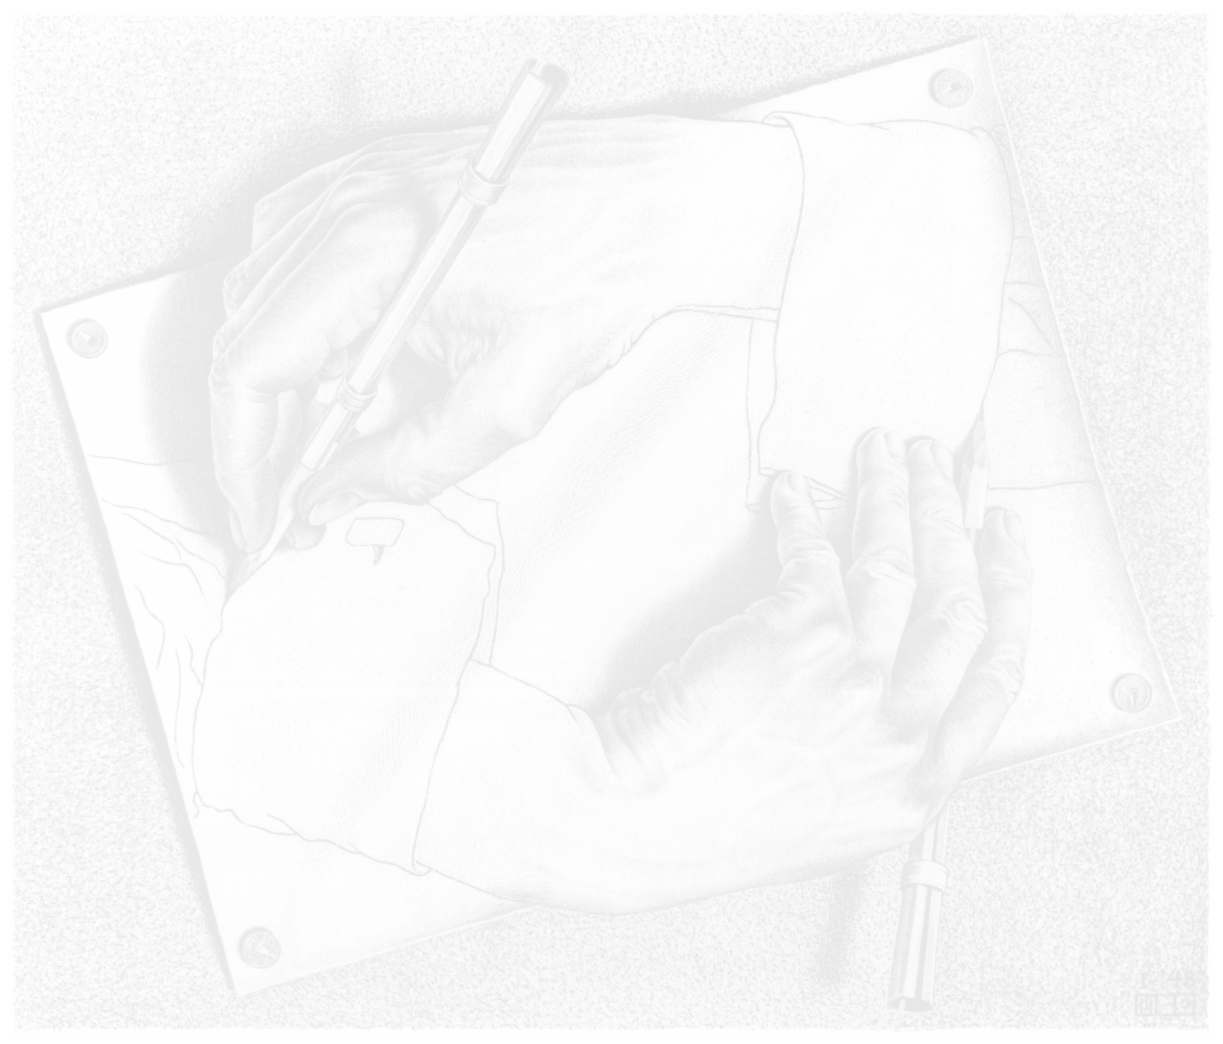
\includegraphics[width=\paperwidth, height=\paperheight]{./figure/escher_hands_tr.png}
%    }
}

%\usetheme{Hannover}
\usetheme{Copenhagen}
\usecolortheme{seahorse}
\usecolortheme{rose}
%\usetheme{Frankfurt}
%\usecolortheme{beetle}

%\useoutertheme[subsection=false]{smoothbars}
%\useoutertheme[subsection=false]{smoothtree}
\useoutertheme{shadow}
\setbeamercovered{dynamic}

\pgfdeclareimage[height=1cm]{logo}{figure/logo}
\logo{\pgfuseimage{logo}}

%\usetikzlibrary{arrows,shapes}
%\tikzstyle{vertex}=[circle,fill=black!25,minimum size=20pt,inner sep=0pt]
%\tikzstyle{selected vertex} = [vertex, fill=red!24]
%\tikzstyle{edge} = [draw,thick,-]
%\tikzstyle{weight} = [font=\small]
%\tikzstyle{selected edge} = [draw,line width=5pt,-,red!50]
%\tikzstyle{ignored edge} = [draw,line width=5pt,-,black!20]


\begin{document}

%%%%%%%%%%%%%%%%%%%%%%%%%%%%%%%%%%%%%%%%%%%%%%%%%%%%%

\begin{frame}
\maketitle
\end{frame}

%%%%%%%%%%%%%%%%%%%%%%%%%%%%%%%%%%%%%%%%%%%%%%%%%%%%%

\begin{frame}
\frametitle{Outline}
	\tableofcontents
\end{frame}

%%%%%%%%%%%%%%%%%%%%%%%%%%%%%%%%%%%%%%%%%%%%%%%%%%%%%

\section{Obiettivi}
\begin{frame}
\frametitle{Obiettivi}

\end{frame}

%%%%%%%%%%%%%%%%%%%%%%%%%%%%%%%%%%%%%%%%%%%%%%%%%%%%%

\begin{frame}
\frametitle{Content-based Recommender System}
Il sistema stabilisce a priori la distanza trai film al fine di raccomandare i più simili alle preferenze dell'utente

\begin{figure}
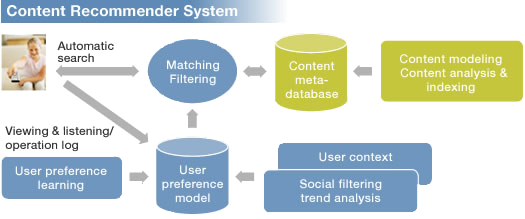
\includegraphics[width=.8\textwidth]{figure/cbrs.png}
\end{figure}

\end{frame}

%%%%%%%%%%%%%%%%%%%%%%%%%%%%%%%%%%%%%%%%%%%%%%%%%%%%%

\begin{frame}
\frametitle{Linked Open Data Cloud}

%
\includegraphics[width=.95\textwidth]{figure/LoDLogo.png}

Collezione (\textbf{Cloud}) di dataset:
\begin{itemize}
\item descritti attraverso RDF
\item fortemente interconnessi fra loro (\textbf{Linked})
\item fruibili liberamente e gratuitamente (\textbf{Open})
\end{itemize}
\end{frame}

%%%%%%%%%%%%%%%%%%%%%%%%%%%%%%%%%%%%%%%%%%%%%%%%%%%%%

\begin{frame}
\frametitle{Resource Description Framework}
Strumento base proposto da \emph{W3C} per la codifica, lo scambio e il riutilizzo di metadati strutturati.

L'RDF Data Model si basa su tre principi chiave:
\begin{enumerate}
\item qualunque cosa può essere identificata da un URI
\item utilizzare il linguaggio meno espressivo per definire qualunque cosa
\item qualunque cosa può dire qualunque cosa su qualunque cosa
\end{enumerate}
\end{frame}

%%%%%%%%%%%%%%%%%%%%%%%%%%%%%%%%%%%%%%%%%%%%%%%%%%%%%

\begin{frame}
\frametitle{Esempio - Resource Description Framework}
Considerando la frase:\\~\\
\begin{center} \emph{Tarantino is the director of the Django Unchained.} \\~\\
\end{center}
L'affermazione può essere suddivisa come: \\~\\
\begin{tabular}{ l | l }
 Soggetto (Risorsa) & Django Unchained \\
 Predicato (Proprietà) & director \\
 Oggetto (Risorsa) & Tarantino \\
\end{tabular}
\end{frame}

%%%%%%%%%%%%%%%%%%%%%%%%%%%%%%%%%%%%%%%%%%%%%%%%%%%%%

\section{Progetto}

\subsection{Sorgente dati}

\begin{frame}
\frametitle{DBPedia}
\begin{columns}

\begin{column}{0.4\textwidth}
\vspace{1cm}
\centering
\includegraphics[width=.8\textwidth]{figure/dbpedialogo}
\begin{itemize}
\item Centro della Linked Open Data Cloud
\item Dump di Wikipedia trasformato in RDF
\end{itemize}
\end{column}
\begin{column}{0.6\textwidth}
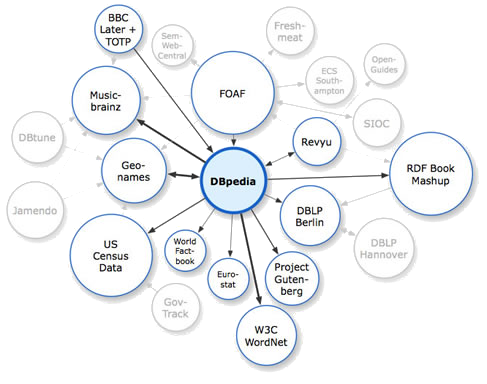
\includegraphics[width=1\textwidth]{figure/AboutDBPedia}
\end{column}
\end{columns}
\end{frame}

%%%%%%%%%%%%%%%%%%%%%%%%%%%%%%%%%%%%%%%%%%%%%%%%%%%%%

\begin{frame}
\frametitle{Proprietà estratte}
Per la raccomandazione di film, abbiamo estratto le seguenti proprietà
\begin{columns}
\begin{column}{0.5\textwidth}
\begin{itemize}
\item studio
\item music
\item music composer
\item writer
\item editing
\item director
\end{itemize}
\end{column}
\begin{column}{0.5\textwidth}
\begin{itemize}
\item subject
\item starring
\item productor
\item writer
\item cinematography
\end{itemize}
\end{column}
\end{columns}
\end{frame}

%%%%%%%%%%%%%%%%%%%%%%%%%%%%%%%%%%%%%%%%%%%%%%%%%%%%%

\section{Conclusioni e sviluppi futuri}
%%%%%%%%%%%%%%%%%%%%%%%%%%%%%%%%%%%%%%%%%%%

\begin{frame}
%	basicstyle=\fontsize{8}{10}\selectfont \ttfamily,%
\begin{center}
Grazie per l'attenzione.
\end{center}
\end{frame}
\end{document}
